\documentclass[10pt,nofootinbib,letterpaper]{revtex4}
%\usepackage[nocap]{ctex}

\usepackage{xeCJK}
% if \usrpackage{xetex} it will invoke the open source Fandol Song Font by default, which lack many Chinese characters
% Linux Requires TrueType Fonts from Windows (locating at C:\Windows\Fonts), and Simlink 
% ln -s blablabla /usr/share/fonts/WindowsFonts 
\setCJKmainfont[BoldFont={SimHei},ItalicFont={KaiTi}]{SimSun}
\setCJKfamilyfont{kaishu}{KaiTi} 
\newcommand*{\kaishu}{\CJKfamily{kaishu}}


\usepackage{amsmath,amssymb,amsfonts,mathrsfs,bm,dsfont}
\usepackage{slashed}
\usepackage{enumerate}
\usepackage{enumitem} % Customize itemize, see https://ctan.org/tex-archive/macros/latex/contrib/enumitem/
\usepackage[all]{xy}
\usepackage[normalem]{ulem}	% delete line
\usepackage{array}
\usepackage{graphics,color}
\usepackage{tikz}
	\usetikzlibrary{calc}
	\usetikzlibrary{decorations.markings}
	\usetikzlibrary{arrows}
	\usetikzlibrary{patterns}
	%\usetikzlibrary{shapes.callouts}
\tikzset{
    level/.style = {
        ultra thick,
        blue,
    },
    connect/.style = {
        dashed,
        red
    },
    label/.style = {
        text width=2cm
    }
}
\usepackage{pgfplots}
%\usepackage[citestyle=authortitle]{biblatex} % able to cite the title, author and year
%\usepackage{hyperref}
\usepackage{feynmp} % feymann diagram
\usepackage{extarrows}
\usepackage[normalem]{ulem} % 文字划掉(横),与 cite 兼容问题,见 https://tex.stackexchange.com/questions/98222/ulem-incompatibility-with-multiple-entries-in-cite

\newcommand*\dd{\mathop{}\!\mathrm{d}}
\newcounter{Claim}[section]
\newenvironment{Claim}[1][]{{\par\normalfont\bfseries \underline{Claim~\stepcounter{Claim}\arabic{Claim}.}~#1~~}}{\par}
\newcounter{Proposition}[section]
\newenvironment{Proposition}[1][]{{\par\normalfont\bfseries \underline{Proposition~\stepcounter{Proposition}\arabic{Proposition}.}~#1~~}}{\par}
\newcounter{Note}[section]
\newenvironment{Note}[1][]{{\par\normalfont\bfseries \underline{Note~\stepcounter{Note}\arabic{Note}.}~#1~~}}{\par}
\newcounter{Lemma}[section]
\newenvironment{Lemma}[1][]{{\par\normalfont\bfseries \underline{Lemma~\stepcounter{Lemma}\arabic{Lemma}.}~#1~~}}{\par}
\newcounter{Corollary}[section]
\newenvironment{Corollary}[1][]{{\par\normalfont\bfseries \underline{Corollary~\stepcounter{Corollary}\arabic{Corollary}.}~#1~~}}{\par}
\newenvironment{Proof}{{\par~{\normalfont\bfseries $\vartriangleright$}~~}}{\hfill $\square$\par\hfill\par} %\par
\newcounter{Def}[section]
\newenvironment{Def}[1][]{{\par\normalfont\bfseries \underline{Definition~\stepcounter{Def}\arabic{Def}.}~#1~~}}{\par}
\newcounter{Assumption}[section]
\newenvironment{Assumption}[1][]{{\par\normalfont\bfseries \underline{Assumption~\stepcounter{Assumption}\arabic{Assumption}.}~#1~~}}{\par}



\allowdisplaybreaks[4] %允许 align 跨页编排

%\def\checkmark{\tikz\fill[scale=0.4](0,.35) -- (.25,0) -- (1,.7) -- (.25,.15) -- cycle;}
%\def\G{\mathcal{G}}
\def\Z{\mathcal{Z}}
\def\H{\mathcal{H}}
\def\D{\mathcal{D}}

\begin{document}
\title{Hall Viscosity --- Adiabatic Evolution of Re-Parameterization}
\author{Xiaodong Hu}
%\altaffiliation[Also at ]{Boson College}
\email{xiaodong.hu@bc.edu}
\affiliation{Department of Physics, Boston College}

\date{\today}

\begin{abstract}
	In this note, we will follow the brilliant work of Avron \cite{avron1995viscosity} to introduce a new kind of topological invaraint of quantum fluids. We generalize the idea of adiabatic evolution of Hamiltonian on the parameter space of flux insertion in the derivation of Hall conductivity to the adiabtic evolutioin of the deformation of the metric (i.e. strain). We show such new parameter sapce is the moduli space of elliptic curves, and the counterpart of Berry curvature can be interpreted as Hall viscosity. It is quantized but no longer an integer.\par
	%\begin{center}
		\hfill\par
		{\centering\kaishu 素月分辉,明河共影,表里俱澄澈。悠然心会,妙处难与君说。\\[0.5em]}
	%\end{center}
	\hfill------ 张孝祥「念奴娇·过洞庭」
\end{abstract}

\maketitle
\tableofcontents

\section{Adiabatic Deformation of the Strain Tensor}
	\subsection{Motivation: Adiabatic Response Theory}
		Given one parameter famility of \emph{quantum} Hamiltonian $H(\bm{R})$ over the curve of the parameter space $\bm{R}:t\mapsto\mathcal{R}$, it is well-known by adiabatic evolution that\footnote{In contrast with Hellmann-Feynman theorem in QM, where the Hamiltonian lives on the $U(1)$-bundle over $[0,1]$, the parameter space here (as base manifold) does not have to be of one-dimensional (although the curve $\bm{R}(t)$ is a one-dimensional submanifold). So in general $(\langle\partial_i n|\dot{n}\rangle-\langle\dot{n}|\partial_i n\rangle)$ is not vanishing.} (by taking the derivative of $\langle n(\bm{R})|H(\bm{R})|n(\bm{R})\rangle=E_n(\bm{R})$ and inserting the Schr\"{o}dinger equation ($\hbar=1$). For detailed discussion, see Sec II. A of \cite{read2011hall})
		\begin{equation}\label{1.1.1}
			\left\langle \dfrac{\partial H}{\partial R^i}\right\rangle=\dfrac{\partial E_n}{\partial R^i}-\Omega_{ij}\dfrac{\dd R^j}{\dd t},
		\end{equation}
		where $\Omega_{ij}\equiv i(\langle\partial_i n|\partial_j n\rangle-\langle\partial_j n|\partial_i n\rangle)$ is the (antisymmetric) Berry curvature of the $U(1)$-bundle over $\mathcal{R}$.\par
		\textbf{By the principle of virtual work, equation \eqref{1.1.1} can also be interpreted as the quantum average of the generalized force related to the variation $\delta R^i$}. This reminds us of the \emph{definition} of the general elastic modulus tensor $\lambda$ and viscosity tensor $\eta$
		\begin{equation}\label{1.1.2}
			\sigma_{\alpha\beta}:=\lambda_{\alpha\beta\gamma\delta}u^{\gamma\delta}-\eta_{\alpha\beta\gamma\delta}\dot{u}^{\gamma\delta}
		\end{equation}
		if we take the stress as the generalized force related to the strain (and it does!), where $\sigma_{\alpha\beta}$ is the stress tensor and $u^{\delta\gamma}$ the symmetric strain tensor
		\begin{equation}\label{1.1.3}
			u^{\delta\gamma}:=\dfrac{1}{2}\left(\dfrac{\partial u^\delta}{\partial x_\gamma}+\dfrac{\partial u^\gamma}{\partial x_\delta}\right), 
		\end{equation}
		with $u^\alpha(\bm{x})$ the local displacement of position $\bm{x}$ along $\alpha$ direction, as is illustrated in FIG.\par
		So if we take the strain to be constant (as the variation $\delta R^i$ does), the adiabatic evolution of such constant strain should give a quantum version of \eqref{1.1.2},
		\begin{equation}\label{1.1.4}
			\left\langle\dfrac{\delta H}{\delta u^{\alpha\beta}}\right\rangle=\dfrac{\delta E}{\delta u^{\alpha\beta}}+\Omega_{\alpha\beta\gamma\delta}\dfrac{\dd u^{\gamma\delta}}{\dd t}.
		\end{equation}
		To give a physical interpretation of \eqref{1.1.4}, one should be clear that the LHS of \eqref{1.1.4} takes average on the \emph{many-body} wave function so is the observable of the \emph{total} stress of the material. While in hydrodynamics, the stress tensor is defined \emph{locally} per volume, so we have the interpretation
		\begin{equation*}
			\sigma_{\alpha\beta}\leftrightarrow\dfrac{1}{V}\left\langle\dfrac{\delta H}{\delta u^{\alpha\beta}}\right\rangle,\quad \lambda_{\alpha\beta\gamma\delta}u^{\gamma\delta}\leftrightarrow\dfrac{1}{V}\dfrac{\delta E}{\delta u^{\alpha\beta}},\quad\eta_{\alpha\beta\gamma\delta}\leftrightarrow\dfrac{\Omega_{\alpha\beta\gamma\delta}}{V},
		\end{equation*}
		or
		\begin{equation}\label{1.1.5}
			\lambda_{\alpha\beta\gamma\delta}=\dfrac{1}{2}\dfrac{\partial^2 E}{\partial u^{\alpha\beta}\partial u^{\gamma\delta}},\quad \eta^A_{\alpha\beta\gamma\delta}=\dfrac{\Omega_{\alpha\beta\delta\gamma}}{V}.
		\end{equation}

	\subsection{Dissipative/Dissipationless Viscosity}
		For a system subjects to isotropic force in equilibrium, the stress tensor is know to be symmetric $\sigma_{ij}=-p\delta_{ij}$. But in general, it contains another part of momentum current that has nothing to do with the momentum transport directly associated with the mass transport \cite{landau1995fluid}
		\begin{equation}\label{1.2.1}
			\sigma_{ij}=-p\delta_{ij}+\sigma_{ij}'.
		\end{equation}
		For isotropic invariant fluids of spatial $d$-dimensional, the most general form of the lowest velocity gradient (contributing to internal friction) we can write down for $\sigma'_{xy}$ is
		\begin{equation}\label{1.2.2}
			\sigma'_{ij}=\eta^{\text{sh}}\left(\dfrac{\partial v_i}{\partial x_j}+\dfrac{\partial v_j}{\partial x_i}-\dfrac{2}{d}\delta_{ij}\dfrac{\partial v_\ell}{\partial x_\ell}\right)+\zeta\delta_{ij}\dfrac{\partial v_\ell}{\partial x_\ell},
		\end{equation}
		where $\eta^{\text{sh}}$ is the \emph{shear viscosity} and $\zeta$ the \emph{bulk viscosity}. Entropy production argument\cite{landau1995fluid}
		\begin{equation}\label{1.2.3}
			k_B T\left(\dfrac{\partial s}{\partial t}+\nabla\cdot \bm{j}_s\right)=\sigma_{ij}'\dfrac{\partial v_i}{\partial x_j}.
		\end{equation}
		requires both viscosities to be non-negative.\par
		Similarly, for stress tensor of the general form \eqref{1.1.2}, we have
		\begin{equation}\label{1.2.4}
			k_B T\left(\dfrac{\partial s}{\partial t}+\nabla\cdot \bm{j}_s\right)=\eta_{\alpha\beta\gamma\delta}\dfrac{\partial u^{\alpha\beta}}{\partial t}\dfrac{\partial u^{\gamma\delta}}{\partial t}.
		\end{equation}
		Splitting the viscosity tensor into symmetric and antisymmetric parts $\eta=\eta^S+\eta^A$. Clearly only the symmetric part is associated with disspation. In fact, for isotropic system $\eta^S$, reduces to exactly the shear viscosity and bulk viscosity we mentioned above.\par
		The antisymmetric part $\eta^A_{\alpha\beta\gamma\delta}\equiv-\eta^A_{\gamma\delta\alpha\beta}$, \textbf{missing from analysis of the usual parity-preserving hydrodynamics}\footnote{See my writing notes.}, however, describes the \emph{non-dissipative response}. Similar to the case of conductivity matrix, Onsager reciprocal relation of time-reversal invariant system plus rotation symmetry require $\eta^A$ to be vanishing. For time-reversal breaking system with rotation invariance (in $(2+1)$-D), we have one-single coefficient of viscosity left,
		\begin{equation}\label{1.2.5}
			\eta^A_{1112}=\eta^A_{1222}=\eta^H,\quad\eta^A_{1122}=0,
		\end{equation}
		 named as \emph{Hall viscosity}.

\section{Example: Free Quantum Hall Fluids on the Torus}
	\subsection{Landau Level on the Torus}
		Taking $m=e=\hbar=1$ for simplicity, the $(2+1)$-D free Hamiltonian of a single charged particle reads
		\begin{equation}\label{2.1.1}
			H=-\dfrac{1}{2}\bigg((\partial_x-iA_x)^2+(\partial_y-iA_y)^2\bigg).
		\end{equation}
		It's convenien to work on complex variable $z\equiv x+iy$ with $\partial_z\equiv\frac{1}{2}(\partial_x-i \partial_y)$, $\partial_{\bar{z}}\equiv\frac{1}{2}(\partial_x+i \partial_y)$, $A_z\equiv\frac{1}{2}(A_x-iA_y)$, and $A_{\bar{z}}\equiv\frac{1}{2}(A_x+iA_y)$. Then by taking the gauge $\bm{A}=(-By,0)$ and introducing the creation and annihilation operator
		\begin{equation*}
			a=i\sqrt{\dfrac{2}{B}}(\partial_{\bar{z}}-iA_{\bar{z}}),\quad a^\dagger=i\sqrt{\dfrac{2}{B}}(\partial_z-iA_z)
		\end{equation*}
		satisfying $[a,a^\dagger]=1$, the above Hamiltonians \eqref{2.1.1} transform into a familiar form of Landau level
		\begin{equation}\label{2.1.2}
			H(B)=B\left(a^\dagger a+\dfrac{1}{2}\right),
		\end{equation}
		with energy $E^{(n)}=B(n+\frac12)$.\par
		The ground state satisfies $a\psi(x,y)=0$. Taking the ansatz $\psi=f(z)g(z,\bar z)$, we have
		\begin{equation*}
			\partial_{\bar z}g(z,\bar z)=i A_{\bar z}g(z,\bar z)=-\dfrac{B}{4}(z-\bar z)g(z,\bar z)\implies g(z,\bar z)=e^{\frac B8(z-\bar z)^2}+h(z)\equiv e^{-\frac B2y^2}+h(z).
		\end{equation*}
		So it takes the form of
		\begin{equation}\label{2.1.3}
			\psi(x,y)\equiv\psi(z,\bar z)=f(z)e^{-\frac B2y^2},
		\end{equation}
		with $f(z)$ some holomorphic function $\partial_{\bar z}f(z)\equiv0$ waiting to be determined.\par
		Symmetry information is helpful in solving the holomorphic function $f(z)$. The original Hamiltonian does not explicitly depends on $x$, so is invariant under $x$-direction translation
		\begin{equation*}
			T_{d_x}^\dagger HT_{d_x}\equiv H,\quad T_{d_x}\equiv e^{id_x\hat{p}_x}\equiv e^{d_x \partial_x}.
		\end{equation*}
		It seems that there is no symmetry along $y$-direction translation. But the extra terms left with BCH formula can be conpensated by an appropriate local $U(1)$ transformation
		\begin{equation*}
			T_{d_y}^\dagger H T_{d_y}\equiv H,\quad T_{d_y}\equiv e^{id_y(\hat{p}_y+B\hat{x}+\phi)}\equiv e^{id_yBx+i\phi}e^{d_y \partial_y}.
		\end{equation*}
		This can be seen from direct calculation
		\begin{equation*}
			T_{d_y}^\dagger(\partial_x+iBy)T_{d_y}=(\partial_x+iBy)+id_y[\hat{p}_y+Bx,\partial_x+iBy]+\cdots=\partial_x+iBy.
		\end{equation*}
		We will choose the global phase $\phi\equiv\frac B2d_xd_y$ for future calculation. Hence we get the \emph{magnetic translation operator}
		\begin{equation}\label{2.1.4}
			T_{\bm{d}}^\dagger HT_{\bm{d}}\equiv H,\quad T_{\bm{d}}\equiv e^{id_yB(x+\frac{d_x}{2})}e^{\bm{d\cdot\partial}}.
		\end{equation}
		If the system is placed on a 2d square with open boundary conditoin, the holomorphic function satisfying the magnetic translation symmetry \eqref{2.1.4} is well-known on the textbook (as Hermitian polynomials). However, as we emphasize before, \textbf{what we want is to exert a constant strain on the whole system. The usual geometric setup with OBC certainly does not fit into our desire}. That's why we try to place such system on the torus $T^2$ as an example instead. This will modify the twisted boundary condition, so making the ground state wave function looks more complicated.

	\subsection{Teichm\"{u}ller Parameterization}
		(Undeformed) torus is usually represented by a rectangle $D=[0,1]\times[0,1]$ with the equivalence relation $z\sim z+1$ and $z\sim z+i$. The standard way to parameterize the constant strain is \emph{Teichm\"{u}ller's deformation of tori} by modifying the periodicity of the parallelogram to $z\sim z+1$ and $z\sim z+\tau$ with $\tau\equiv\tau_1+i\tau_2$ a complex number. When $\tau=i$, we get back to the original undeformed torus.\par
		Under Teichm\"{u}ller parameterization, the ground state wave function must satisfy
		\begin{equation}\label{2.2.1}
			T_{(1,0)}\psi(x,y)\equiv\psi(x,y),\quad T_{(\tau_1,\tau_2)}\psi(x,y)\equiv\psi(x,y).
		\end{equation}
		Inserting the expression of magnetic translation operator, we have
		\begin{equation}\label{2.2.2}
			\psi(x+1,y)\equiv\psi(x,y),\quad \psi(x+\tau_1,y+\tau_2)e^{i\tau_2B(x+\frac{\tau_2}{2})}\equiv\psi(x,y).
		\end{equation}
		For consistensy, the translation $(x,y)\mapsto(x+1,y)\mapsto(x+1+\tau_1,y+\tau_2)$ and $(x,y)\mapsto(x+\tau_1,y+\tau_2)\mapsto(x+\tau_1+1,y+\tau_2)$ must commute, giving exactly the \textbf{Dirac quantization of magnetic field} 
		\begin{equation}\label{2.2.3}
			e^{i\tau_2B}\equiv1=e^{i2\pi N}\implies B=\dfrac{2\pi N}{\tau_2},\quad N\in\mathbb{N}.
		\end{equation}
		And the energy of Landau level reads
		\begin{equation}\label{2.2.4}
			E^{(n)}(\tau)=\dfrac{2\pi N}{\tau_2}\left(n+\dfrac{1}{2}\right).
		\end{equation}
		Another way to prove \eqref{2.2.3} is to place a Dirac particle on the torus and invoke the Atiyah-Singer theorem, cf. \cite{levay1995berry}.\par

		Substituting the ansatz of ground state wave function \eqref{2.1.3}, we get
		\begin{equation}\label{2.2.5}
			f(z+1)\equiv f(z),\quad f(z+\tau)\equiv f(z)e^{i2\pi N(z-\frac{\tau}{2})}.
		\end{equation}
		The holomorphic functions that satisfy the above twisted boundary condition is the \emph{Jacobi theta function with rational characteristics} \cite{wen2012modular}
		\begin{equation}\label{2.2.6}
			f_\ell(z|\tau)\equiv\vartheta\left[\begin{array}{c}
				\ell/N\\0
			\end{array}\right](Nz|N\tau)\equiv\sum_{m=-\infty}^\infty e^{i\pi\tau(m+\ell/N)^2+i2\pi(m+\ell/N)Nz}.
		\end{equation}
		$f(z)$ has $N$ independent components labeled by $\ell=0,1,2,\cdots,N$, so \textbf{the Landau level on deformed torus is still $N$-fold degenerated}.\par
		Given the ground state wave function, we could immediately work out the Berry connection and Berry curvature in principle. But in light of the complicated normalization condition of the theta functions and physical ambiguity of the brute-force calculation, we would better choose to work in another way.

	\subsection{Inclined Coordinates and $\mathfrak{so}(2,1)$ Symmetry}
		One must be aware that the above Teichm\"{u}ller parameterization $\tau=\tau_1+i\tau_2$, appearing in reparameterization of the complex structure of the world sheet in string theory, encodes \emph{both} deformation of shearing and scaling of our torus. However, \textbf{\color{red}in order to isolate each component of the adiabatic evolution, we prefer to use $\tau=\tau_1+i\tau_2$ to encode solely the area-preserving deformation, while use another parameter $V\equiv\sqrt{\det g_{\mu\nu}}$ to encode the scaling deformation (so we are working with a NEW parameterization)}. This can be achieved by introducing a global scaling factor after transforming into the inclined coordinates $\{\theta_1,\theta_2\}$
		\begin{equation*}
			z\equiv x+iy=\sqrt{\dfrac{V}{\tau_2}}(\theta_1+\tau\theta_2),
		\end{equation*}
		or $x\mapsto\sqrt{V/\tau_2}(\theta_1+\tau_1\theta_2)$ and $y\mapsto\sqrt{V\tau_2}\theta_2$, with the metric $g=g_{\mu\nu}\dd x^\mu\otimes\dd x^\nu=g_{ab}\dd\theta^a\otimes\dd\theta^b$ where
		\begin{equation*}
			g_{ab}=\dfrac{V}{\tau_2}\left(\begin{array}{cc}
				1&\tau_1\\\tau_1&|\tau|^2
			\end{array}\right).
		\end{equation*}
		The pre-factor is added to ensure the coefficient of the volume form to be invariant $\sqrt{\det g_{\mu\nu}}=\sqrt{\det g_{ab}}=V$ under any value of $\tau$ so meet our desire of the isolated parameterization of the deformation.\par
		One should be aware that the new parameterization changes the periodicity to $z\sim z+\sqrt{V/\tau_2}$ and $z\sim z+\sqrt{V/\tau_2}\tau$, so the above analysis of magnetic translation will alter the Dirac quantization condition to
		\begin{equation}\label{2.3.0}
			B(\tau_1,\tau_2,V)=B(V)=\dfrac{2\pi N}{V},
		\end{equation}
		while remaining the form of the Landau level energy $E^{(n)}=B(V)(n+\frac12)$.\par
		Now in the new coordinates the Hamiltonian reads
		\begin{equation}\label{2.3.1}
			H(V,\tau_1,\tau_2,\phi_1,\phi_2)\equiv\dfrac{-1}{2}g^{\mu\nu}D_\mu D_\nu=\dfrac{-1}{2V\tau_2}\bigg[|\tau|^2D_1^2-\tau_1(D_1 D_2+D_2D_1)+D_2^2\bigg],
		\end{equation}
		where $D_a\equiv\partial/\partial\theta^a-iA_a$, and 
		\begin{equation*}
			\mathcal{A}\equiv A_\mu\dd x^\mu\equiv A_a\dd\theta^a\implies A_1=-BV\theta_2, A_2=-BV\theta_2\tau_1.
		\end{equation*}
		For futher discussion, we would like to insert by hand another two fluxes\footnote{In our unit, each $\phi_a$ carries $2\pi$ numbers of the magnetic flux quanta $hc/e$.} $\phi_1$ and $\phi_2$ for each kinds of circle of the torus. Then
		\begin{equation*}
			D_1=\dfrac{\partial }{\partial\theta_1}+i(BV\theta_2+\phi_1),\quad D_2=\dfrac{\partial}{\partial \theta_2}+i(BV\theta_2\tau_1+\phi_2),
		\end{equation*}
		and the Hamiltonian becomes a five-parameter family $H(V,\tau_1,\tau_2,\phi_1,\phi_2)$. Each of them gives one component of the adiabatic evolution.\par
		The two differential operators in \eqref{2.3.1} can be re-arranged to display a new symmetry that will simplify our calculation. By assigining a vector \cite{levay1995berry}
		\begin{equation}\label{2.3.2}
			X_1\equiv\dfrac{1-|\tau|^2}{2\tau_2},\quad X_2\equiv\dfrac{\tau_1}{\tau_2},\quad X_3\equiv\dfrac{1+|\tau|^2}{2\tau_2},
		\end{equation}
		on a flat three-dimensional space with the Lorentzian metirc $h_{\mu\nu}=\mathop{\mathrm{diag}}(1,1,-1)$ (then vector $\bm{X}$ is normalized $\bm{X}\cdot\bm{X}\equiv-1$), we can write the Hamiltonian as
		\begin{equation}\label{2.3.3}
			H(\bm{X})=\dfrac{1}{2\lambda V}(X_1J_1+X_2J_2-X_3J_3)\equiv\dfrac{1}{2\lambda V}\bm{X}\cdot\bm{J}
		\end{equation}
		with
		\begin{equation*}
			J_1\equiv\lambda(D_1^2-D_2^2),\quad J_2=\lambda(D_1D_2+D_2D_1),\quad J_3=\lambda(D_1^2+D_2^2).
		\end{equation*}
		Using the fact $[D_1,D_2]\equiv-iBV$, we can choose the constant $\lambda\equiv1/4BV$ to construct a $\mathfrak{so}(2,1)$ Lie algebra 
		\begin{equation}\label{2.3.4}
			[J_1,J_2]=-iJ_3,\quad[J_2,J_3]=iJ_1,\quad[J_3,J_1]=iJ_2.
		\end{equation}
		When $\tau=i$, i.e., going back to the undeformed torus, we have $\bm{X}=(0,0,1)$. \textbf{So the deformed Hamiltonian (parameterized by $\tau$ and $V$) and undeformed Hamiltonian are connected just by a unitary rotation of the $\bm{J}$ space}. In terms of the polar coordinate $X_1\equiv\sinh\theta\cos\phi$, $X_2\equiv\sinh\theta\sin\phi$, and $X_3\equiv\cosh\theta$, we can write
		\begin{equation}\label{2.3.5}
			H(\bm{X})=\mathcal{U}(\theta,\phi)H(X_3=1)\mathcal{U}^{-1}(\theta,\phi),
		\end{equation}
		where $H(X_3=1)=2BX_3J_3$ and $\mathcal{U}(\theta,\phi)\equiv e^{-i\theta(\sin\phi J_1-\cos\phi J_2)}$.\par
		The original $N$-fold ground state eigenstates of the undeformed Hamiltonian, denoting as $|\phi_\ell(X_3=1)\rangle$, has NO dependence on the Teichm\"{u}ller parameter $\tau$, thus \textbf{the adiabatic evolution of the deformation is fully encoded in the unitary operator $\mathcal{U}(\theta,\phi)$}. More explicitly, for the connection one-form, we have \cite{levay1993algebraic}
		\begin{align}
			\mathcal{A}_{\ell\ell'}&\equiv i\langle\phi_\ell(\tau)|\dd|\phi_{\ell'}(\tau)\rangle\nonumber\\
			&=i\langle\phi_\ell(X_3=1)|\mathcal{U}^{-1}\dd\mathcal{U}|\phi_{\ell'}(X_3=1)\rangle=i\langle\phi_\ell(X_3=1)|\mathcal{U}^{-1}\nabla_{\bm{X}}\mathcal{U}\dd\bm{X}|\phi_{\ell'}(X_3=1)\rangle\nonumber\\
			&=i\left\langle\phi_\ell(X_3=1)\middle|\sum_{i,k}\omega_{ik}J_k\dd X_i\middle|\phi_{\ell'}(X_3=1)\right\rangle,\label{2.3.6}
		\end{align}
		where in the last line we expanded the coefficients of the Maurer-Cartan $1$-form in terms of $\{\bm{J}\}$. Since $\omega_i^k$ are representation-independent, we will choose a faithful representation $(J_1,J_2,J_3)=(\sigma_1/2i,\sigma_2/2i,\sigma_3/2)$ for simplicity. Furthermore, using the ground state energy of the deformed torus \eqref{2.2.4} (it is certainly coordinate-independent) and the fact $H(X_3=1)\equiv 2BX_3J_3$, we immediately have
		\begin{equation*}
			J_3|\phi_\ell(X_3=1)\rangle=\dfrac{1}{2}\left(n+\dfrac{1}{2}\right)|\phi_\ell(X_3=1)\rangle,
		\end{equation*}
		with $n$ labeling the energy levels as usual. Therefore
		\begin{align*}
			\mathcal{A}_{\ell\ell'}&=i\left\langle\phi_\ell(X_3=1)\middle|\left(\begin{array}{cc}
				\frac{i}{2}(\cosh\theta-1)\dd\phi & \frac{1}{2}e^{-i\phi}(i\dd\theta+\sinh\theta\dd\phi) \\[0.8em]
				\frac{1}{2}e^{i\phi}(-i\dd\theta+\sinh\theta\dd\phi) & \frac{i}{2}(1-\cosh\theta)\dd\phi
			\end{array}\right)\middle|\phi_{\ell'}(X_3=1)\right\rangle\\
			&=i\left\langle\phi_{\ell}(X_3=1)\middle|i(\cosh\theta-1)J_3\middle|\phi_{\ell'}(X_3=1)\right\rangle\dd\phi\\
			&=-(\cosh\theta-1)\times\dfrac{1}{2}\left(n+\dfrac{1}{2}\right)\delta_{\ell\ell'}\dd\phi,
		\end{align*}
		where in the second line only the $J_3$ component of the $2\times2$ matrix survives in the evaluation of the expectation value because $|\phi_\ell(X_3=1)\rangle$ are the eigenstates of $J_3$, while $J_1$ and $J_2$ plays the role of ladder operators. Finally, for ground states $n=0$, we can re-express the polar coordinate $\{\theta,\phi\}$ in terms of Cartestian coordinate $\bm{X}$, and then the Teichm\"{u}ller parameter as
		\begin{equation}\label{2.3.6}
			\mathcal{A}_{\ell\ell'}=\delta_{\ell\ell'}\dfrac{1}{4}(1-\cosh\theta)\dd\phi\equiv\delta_{\ell\ell'}\dfrac{1}{4}\dfrac{X_2\dd X_1-X_1\dd X_2}{1+X_3}\equiv-\delta_{\ell\ell'}\dfrac{\dd\tau_1}{4\tau_2}.
		\end{equation}
		So the curvature $2$-form of the deformation reads
		\begin{equation}\label{2.3.7}
			\mathcal{F}\equiv \dd\mathcal{A}=\dfrac{\dd\tau_1\wedge\dd\tau_2}{4\tau_2^2}.
		\end{equation}

\section{Geometrical and Physical Meaning of Hall Viscosity}
	\subsection{Adiabatic Equations of Motion}
		The ground state energy of a single electron is $E=B/2$. So for a fully-filled Landau level of $N$ degeneracy, the total energy is only the single-variable function of $V$
		\begin{equation}\label{3.1.1}
			E(V,\tau_1,\tau_2,\phi_1,\phi_2)=\dfrac{BN}{2}=\dfrac{2\pi N^2}{V},
		\end{equation}
		telling that the corresponding modulus tensor has only ONE non-vanishing component\footnote{Note here we do not write the modulus tensor $\lambda_{\alpha\beta\gamma\delta}$ in components of the strain tensor $u_{\alpha\beta}$ as its definition requires, but in components of the independent displacement vectors. However, the conclusion that only one component of modulus tensor survives would not change if we write in the former form.}
		\begin{equation}\label{3.1.2}
			\lambda_{VV}\equiv\dfrac{1}{2}\dfrac{\partial^2 E}{\partial V^2}=\dfrac{2\pi N}{V^3}.
		\end{equation}
		\textbf{\color{red}This is consistent with our expectation of a quantum \emph{fluid}: there is only one component of a longitudinal sound wave; the other two transverse modes should be soft in fluids}.\par
		The total non-vanishing curvature $2$-form (including the familiar one coming from flux insertion) of the $\ell$-th eigenstate is
		\begin{equation}\label{3.1.3}
			\Omega^\ell=\dfrac{\dd\tau_1\wedge\dd\tau_2}{4\tau_2^2}-\dfrac{1}{B}\dd\phi_1\wedge\dd\phi_2.
		\end{equation}
		So the left four transport EOM of a fully-filled Landau level (of $N$ degeneracy) reads
		\begin{align*}
			\left\langle \dfrac{\partial H}{\partial V}\right\rangle&=\dfrac{2\pi N}{V^2}+0,\\
			\left\langle \dfrac{\partial H}{\partial \tau_1}\right\rangle&=0+\dfrac{N}{4\tau_2^2}\dfrac{\dd\tau_2}{\dd t},\\
			\left\langle \dfrac{\partial H}{\partial \tau_2}\right\rangle&=0-\dfrac{N}{4\tau_2^2}\dfrac{\dd\tau_2}{\dd t},\\
			\left\langle \dfrac{\partial H}{\partial \phi_1}\right\rangle&=0-\dfrac{N}{B}\dfrac{\dd\phi_2}{\dd t},\\
			\left\langle \dfrac{\partial H}{\partial \phi_2}\right\rangle&=0+\dfrac{N}{B}\dfrac{\dd\phi_1}{\dd t}.
		\end{align*}
		To interprete the first part of the curvature \eqref{3.1.3} as Hall viscosity, we have to re-write the $2$-form of deformation parameters in terms of the $2$-form of the strain tensor. In our new \emph{inclined} coordinate $\{\theta_1,\theta_2\}$, the infinitesimal displacement vector parameterized by $\{V,\tau_1,\tau_2\}$ takes the form of
		\begin{align*}
			\dd u^1(\theta_1,\theta_2)&\equiv\dd \left(\sqrt{\dfrac{V}{\tau_2}}(\theta_1+\tau_1\theta_2)\right) =\dfrac{1}{2}\sqrt{\dfrac{V}{\tau_2}}\left(\dfrac{\dd V}{V}-\dfrac{\dd\tau_2}{\tau_2}\right)(\theta_1+\tau_1\theta_2)+\sqrt{\dfrac{V}{\tau_2}}\dd\tau_1\theta_2,\\
			\dd u^2(\theta_1,\theta_2)&\equiv\dd \left(\sqrt{V\tau_2}\theta_2\right)=\dfrac{1}{2}\sqrt{\dfrac{V}{\tau_2}}\left(\dd\tau_1+\dfrac{\tau_2}{V}\dd V\right)\theta_2.
		\end{align*}

		\noindent But what we want is the Hall viscosity in the undeformed coordinate
		\begin{equation*}
			\begin{cases}
				\widetilde{x}\equiv\sqrt{V/\tau_2}(\theta_1+\tau_1\theta_2),\\[0.8em]
				\widetilde{y}\equiv\sqrt{V\tau_2}\theta_2.
			\end{cases}
		\end{equation*}
		Namely,
		\begin{align*}
			\dd u^1(\widetilde{x},\widetilde{y})&=\dfrac{1}{2}\left(\dfrac{\dd V}{V}-\dfrac{\dd\tau_2}{\tau_2}\right)\widetilde{x}+\dfrac{\dd\tau_1}{\tau_2}\widetilde{y},\\
			\dd u^2(\widetilde{x},\widetilde{y})&=\dfrac{1}{2}\left(\dfrac{\dd\tau_1}{\tau_2}+\dfrac{\dd V}{V}\right)\widetilde{y}.
		\end{align*}
		Thus the infinitesimal strain tensor
		\begin{align*}
			\dd u_{11}&\equiv\dfrac{1}{2}\left(\dfrac{\partial\dd u^1}{\partial \widetilde{x}}+\dfrac{\partial\dd u^1}{\partial \widetilde{x}}\right)=\dfrac{1}{2}\left(\dfrac{\dd V}{V}-\dfrac{\dd\tau_2}{\tau_2}\right),\\
			\dd u_{12}&\equiv\dfrac{1}{2}\left(\dfrac{\partial\dd u^1}{\partial \widetilde{y}}+\dfrac{\partial\dd u^2}{\partial \widetilde{x}}\right)=\dfrac{1}{2}\dfrac{\dd\tau_1}{\tau_2},\\
			\dd u_{22}&\equiv\dfrac{1}{2}\left(\dfrac{\partial\dd u^2}{\partial \widetilde{y}}+\dfrac{\partial\dd u^2}{\partial \widetilde{y}}\right)=\dfrac{1}{2}\left(\dfrac{\dd V}{V}+\dfrac{\dd\tau_2}{\tau_2}\right).
		\end{align*}
		And the Berry curvature of a fully-filled landau level becomes
		\begin{equation}\label{3.1.4}
			\Omega=\dfrac{N}{2}(\dd u_{11}-\dd u_{22})\wedge\dd u_{12}-\dfrac{N}{B}\dd\phi_1\wedge\dd\phi_2.
		\end{equation}
		Following \eqref{1.1.5} we obtain the viscosity tensor consistent with the symmetry argument
		\begin{equation}\label{3.1.5}
			\eta^H\equiv\eta^A_{1112}=\eta^A_{1222}=\dfrac{N}{4V}\equiv\dfrac{1}{4}\bar{n},\quad\eta^A_{1122}=0,
		\end{equation}
		and recover the familiar conductivity tensor (Recall that for the variation of fluxes, the generalized force $-\partial H/\partial \phi_a$ has the meaning of current operator, and the generalized velocity $\dot{\phi}_a$ has the meaning of electromotive force, so the coefficient has exactly the meaning of the Hall conductivity)
		\begin{equation}\label{3.1.6}
			\sigma_{12}=\dfrac{N}{BV}=\dfrac{1}{2\pi},\quad\sigma_{11}=0.
		\end{equation}
		\indent The result \eqref{3.1.5}, quantized up to a constant, is a special case of the celebrated expression (with the units recovered) of a general consideration \cite{read2011hall}
		\begin{equation}\label{3.1.7}
			\eta^H=\dfrac{1}{2}\bar{n}\bar{s}\hbar
		\end{equation}
		with the ``orbital spin'' of one-half (it is the quantized angular momentum of cyclotron motion $(n+\frac12)$ that takes the position of orbital spin here, and we have taken the ground state $n=0$).

	\subsection{Parameter Space of the Deformation}
		Recognizing the second part of \eqref{3.1.3} as the (flat) volume form of the parameter space of flux insertion (still a torus, but do not get confused with the base manifold of our example), then Niu \textit{et al.} \cite{niu1985quantized} tells that the integration of the Berry curvature gives the Chern number (as an integer) of the $U(1)$-boundle over such torus.\par
		In the same spirit, \textbf{\color{red}we can interprete the first part of \eqref{3.1.3} as the volume form of the parameter space of deformation $\mathcal{M}$, and expect the integration of it give rise to another topological invariant as the Chern number of the $U(1)$-bundle over $\mathcal{M}$}.\par
		But the question is, what is the space $\mathcal{M}$ (locally represented by $\tau_1$ and $\tau_2)$? Recall in string theory that the study of Teichm\"{u}ller parameterization $z=x+\tau y$ tells another \emph{large coordinate transformation} that cannot be obtained by successive infinitesimal transformation
		\begin{equation*}
			\left(\begin{array}{c}
				x'\\y'
			\end{array}\right)=M\left(\begin{array}{c}
				x\\y
			\end{array}\right),\quad M\equiv\left(\begin{array}{cc}
				a&b\\c&d
			\end{array}\right)\in\mathrm{SL}(2,\mathbb{Z}),
		\end{equation*}
		or $z=x+\tau y=x'+\tau'y'$ such that 
		\begin{equation*}
			\tau'=\dfrac{a\tau+b}{c\tau+d}.
		\end{equation*}
		\indent Similarly, in our parameterization where the Hamiltonian takes the form of a five-parameter family $H(V,\tau_1,\tau_2,\phi_1,\phi_2)$, the above modular transformation changes the Hamiltonian into $H(V,\tau_1',\tau_2',\phi_1',\phi_2')$ with $\tau'$ defined above and
		\begin{equation*}
		 	\phi_1'=d\phi_1+b\phi_2,\quad \phi_2'=c\phi_1+a\phi_2.
		\end{equation*}
		This means that \textbf{\color{red}the \emph{family} of the Hamiltonian of zero flux $H(V,\tau_1,\tau_2,0,0)$ is invariant under modular transformation $\mathrm{SL}(2,\mathbb{Z})$. Thus the parameter space $\mathcal{M}$ labeled by $\{\tau_1,\tau_2\}$ coincides with nothing but the \emph{moduli space of elliptic curves} in algebraic geometry}. Each point of $\mathcal{M}$ represent one characteristic of the orbit of the Hamiltonian under the action of $\mathrm{SL}(2,\mathbb{Z})$. So $\mathcal{M}$ can be represent by the \emph{foundamental domain} $F$ of the modular group $\mathrm{SL}(2,\mathbb{Z})$, see in FIG. \ref{fig:FD},
		\begin{figure}[!htp]
			\centering
			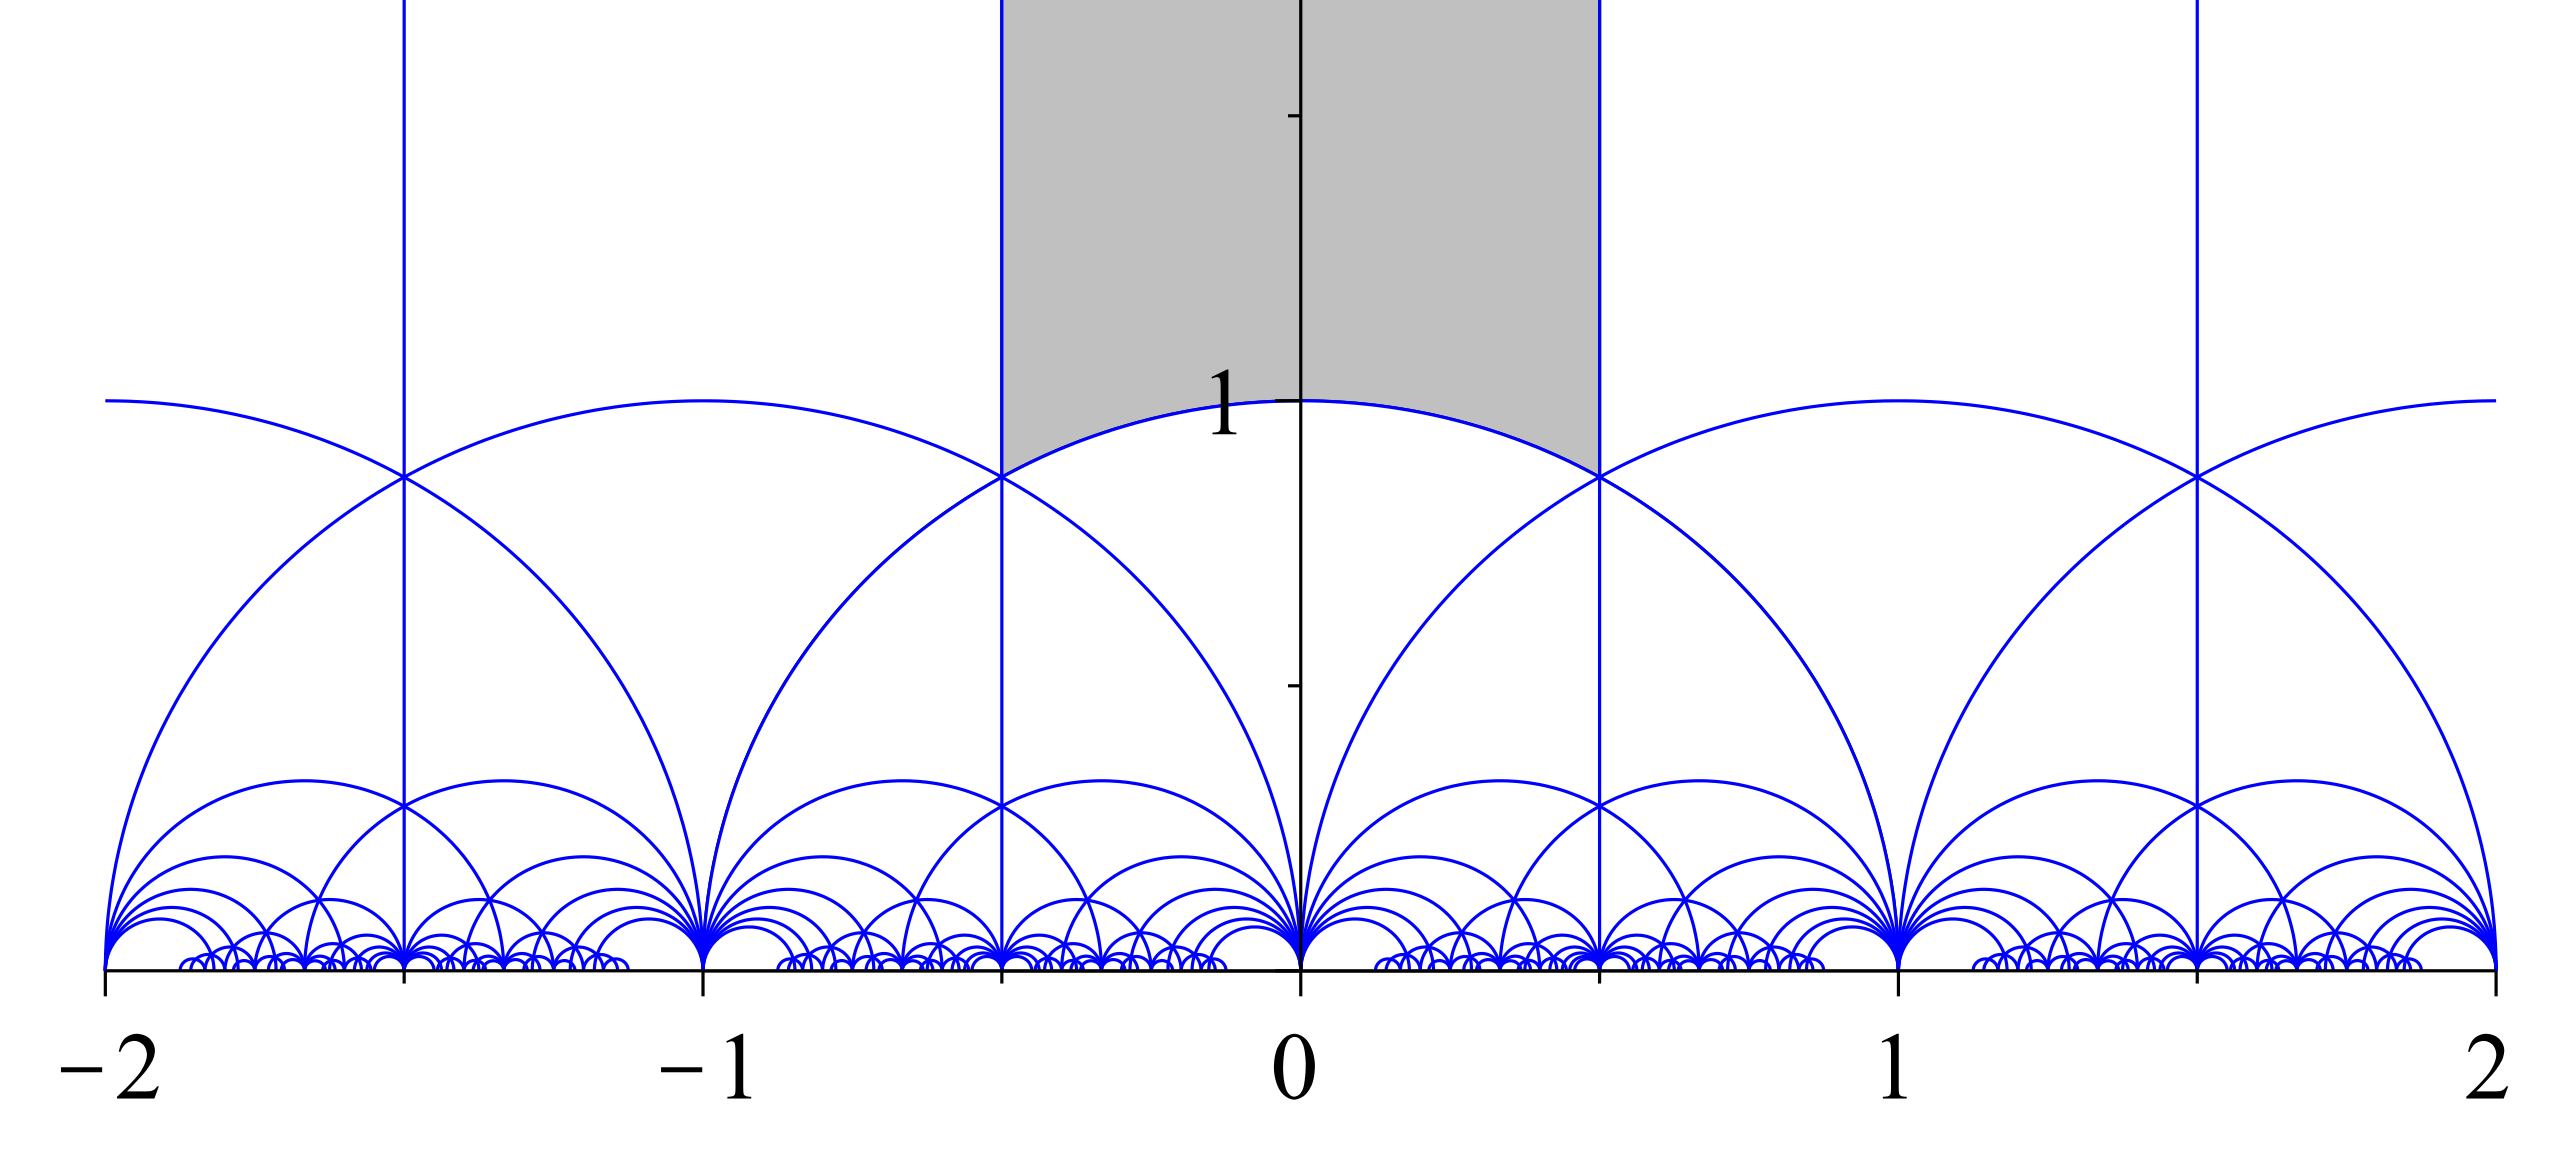
\includegraphics[scale=0.15]{SL2.png}
			\caption{Fundamental Domain of the Modular Group}
			\label{fig:FD}
		\end{figure}
		whose volume is known\footnote{See, for example, \url{https://math.stackexchange.com/questions/30502/hyperbolic-area-and-sl-2}.}
		\begin{equation}\label{3.2.1}
			\int_F\dfrac{\dd\tau_1\wedge\dd\tau_2}{\tau_2^2}=\dfrac{\pi}{3}.
		\end{equation}
		Therefore the integration of the viscous Berry curvature over the moduli space $\mathcal{M}$ (or fundamental domain $F$) is
		\begin{equation}\label{3.2.2}
			\dfrac{1}{2\pi}\int_F\Omega^{\text{vis}}\equiv\dfrac{1}{2\pi}\int_F\dfrac{N}{4}\dfrac{\dd\tau_1\wedge\dd\tau_2}{\tau_2^2}=\dfrac{N}{24}.
		\end{equation}
		Such topological Chern number (in the orbifold sense) is no longer an integer as the Chern number of $U(1)$-bundle should be. This is not surprising, because the moduli space (parameter space of deformation) is not compact.


\bibliography{hxd}
\bibliographystyle{apsrev} % apsrev is format for PRL of APS
\end{document}